\section{Régimen de Volatilidad Estructural e Ilusión del Efecto Base}

% ================================================================
\begin{frame}{Riesgo Regional: Enclaves Exhiben $4.4\times$ Más Volatilidad}
\vspace{-0.18cm}
\begin{center}
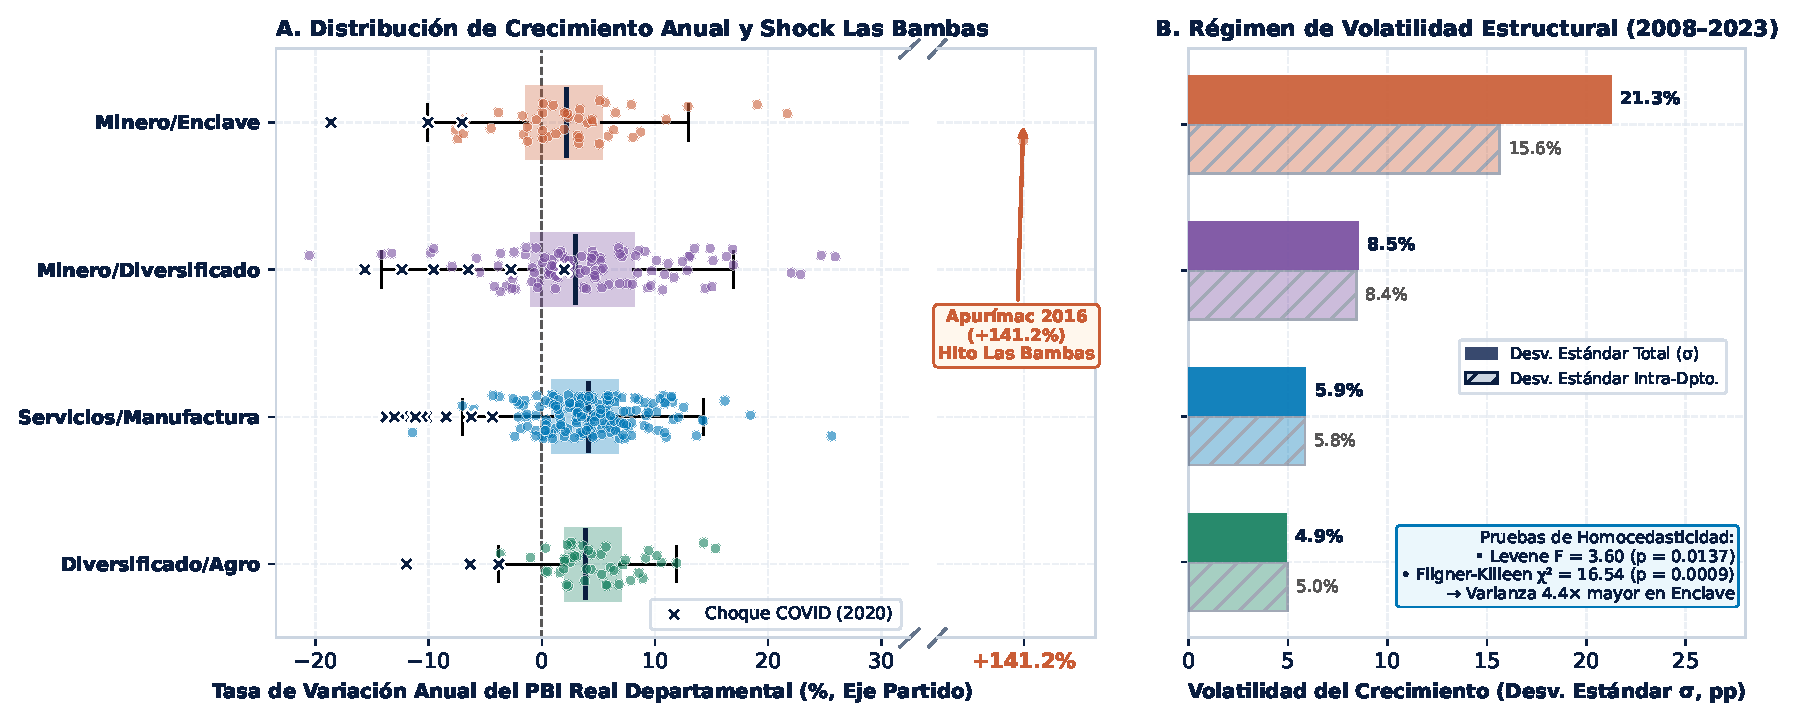
\includegraphics[width=0.89\textwidth,height=0.47\textheight,keepaspectratio]{figures/fig4_volatilidad_estructural.pdf}
\end{center}
\vspace{-0.24cm}
\begin{columns}[T,onlytextwidth]
\begin{column}{0.56\textwidth}
\begin{ccdebox}[left=2mm,right=2mm,top=0.8mm,bottom=0.8mm]
\scriptsize\RaggedRight
\textbf{Heterocedasticidad verificada}: El test de \textbf{Levene} ($F=3.97, p=0.0083$) y \textbf{Fligner-Killeen} ($\chi^2=17.54, p=0.0005$) confirman varianzas dispares ($\sigma = 20.5\%$ en Enclave vs.\ $4.6\%$ en Agro).
\end{ccdebox}
\end{column}
\begin{column}{0.41\textwidth}
\begin{keybox}[left=2mm,right=2mm,top=0.8mm,bottom=0.8mm]
\scriptsize\RaggedRight \textbf{Shock Las Bambas (2016)}: Apurímac creció $+141.2\%$ en un año, inflando la varianza residual en tasas.
\end{keybox}
\end{column}
\end{columns}
\source{Panel 2008--2025 ($N=428$). Pruebas de varianza ejecutadas en \texttt{modelo-econometrico.ipynb}.}
\end{frame}

% ================================================================
\begin{frame}{El Puzzle de las Tasas Anuales (Modelos M1--M4)}
\vspace{-0.14cm}
\begin{columns}[T,onlytextwidth]
\begin{column}{0.56\textwidth}
\begin{ccdebox}[left=2mm,right=2mm,top=1.1mm,bottom=1.1mm]
\scriptsize
\textbf{\textcolor{ccdenavy}{Panel FE sobre Crecimiento Anual ($\text{var\_pib}_{it}$, 2008--2025)}}
\vspace{0.04cm}

\resizebox{\linewidth}{!}{%
\renewcommand{\arraystretch}{1.10}
\begin{tabular}{@{}l r r r r@{}}
\toprule
\textbf{Variable / Estadístico} & \textbf{M1 ($K=4$)} & \textbf{M2 (Macro)} & \textbf{M3 (+Rebote)} & \textbf{M4 (Sin Apu16)} \\
\midrule
Intercepto ($\hat{\alpha}$) & $4.53^{***}$ & $4.53^{***}$ & $4.12^{***}$ & $4.19^{***}$ \\
$\text{COVID}_{2020}$ (Base) & $-11.95^{***}$ & $-14.43^{***}$ & $-13.97^{***}$ & $-14.43^{***}$ \\
$\text{REBOTE}_{2021}$ (Base) & --- & --- & $+7.80^{***}$ & --- \\
\midrule
$\text{COVID} \times \text{Serv./Manuf.}$ & $-2.90$ (0.20) & --- & --- & --- \\
$\text{COVID} \times \text{Minero/Div.}$ & $-1.70$ (0.64) & --- & --- & --- \\
$\text{COVID} \times \text{Minero/Enclave}$ & $-5.73$ (0.13) & --- & --- & --- \\
$\text{COVID} \times \text{Macro Minero}$ & --- & $-0.63$ (0.81) & $-0.75$ (0.77) & $+0.28$ (0.91) \\
$\text{REBOTE} \times \text{Macro Minero}$ & --- & --- & $-2.11$ (0.45) & --- \\
\midrule
Observaciones ($N$) & 428 & 428 & 428 & 427 \\
$R^2$ Within & 0.1390 & 0.1376 & 0.1691 & \textcolor{okgreen}{\textbf{0.2620}} \\
Poolability $F$ ($p$-valor) & 0.96 (0.51) & 0.92 (0.57) & 0.96 (0.52) & 1.07 (0.38) \\
\bottomrule
\end{tabular}%
}
\vspace{0.02cm}
{\tiny Nota: $p$-valores con errores estándar clusterizados entre paréntesis. $^{***}p<0.01$.}
\end{ccdebox}
\end{column}

\begin{column}{0.41\textwidth}
\begin{contrastbox}{warn}{Diagnóstico del Puzzle}
\scriptsize\RaggedRight
\begin{enumerate}\setlength{\itemsep}{0.10em}
  \item \textbf{Parálisis transversal (Q2-2020):} El confinamiento detuvo tanto la gran minería como el comercio ($\approx -14.4\%$).
  \item \textbf{Ruido pre-pandemia:} En M4, excluir solo \textit{Apurímac 2016} casi duplica el $R^2_{\text{within}}$ ($13.8\% \rightarrow 26.2\%$).
  \item \textbf{Ilusión del efecto base:} Caer $-12\%$ en 2020 y crecer $+9\%$ en 2021 luce positivo en $\text{var\_pib}$, pero deja al PIB en $95.9\%$ del nivel de 2019.
\end{enumerate}
\end{contrastbox}
\vspace{0.04cm}
\begin{keybox}[left=2mm,right=2mm,top=0.8mm,bottom=0.8mm]
\scriptsize\RaggedRight \textbf{Solución}: Modelar el \textbf{nivel acumulado indexado ($\text{PIB}_{2019=100}$)}.
\end{keybox}
\end{column}
\end{columns}
\source{Estimaciones con \texttt{linearmodels.PanelOLS} en \texttt{econ\_paso1.py} a \texttt{econ\_paso3.py}.}
\end{frame}

